%  A simple AAU report template.
%  2015-05-08 v. 1.2.0
%  Copyright 2010-2015 by Jesper Kjær Nielsen <jkn@es.aau.dk>
%
%  This is free software: you can redistribute it and/or modify
%  it under the terms of the GNU General Public License as published by
%  the Free Software Foundation, either version 3 of the License, or
%  (at your option) any later version.
%
%  This is distributed in the hope that it will be useful,
%  but WITHOUT ANY WARRANTY; without even the implied warranty of
%  MERCHANTABILITY or FITNESS FOR A PARTICULAR PURPOSE.  See the
%  GNU General Public License for more details.
%
%  You can find the GNU General Public License at <http://www.gnu.org/licenses/>.
%
%  A simple AAU report template.
%  2015-05-08 v. 1.2.0
%  Copyright 2010-2015 by Jesper Kjær Nielsen <jkn@es.aau.dk>
%
%  This is free software: you can redistribute it and/or modify
%  it under the terms of the GNU General Public License as published by
%  the Free Software Foundation, either version 3 of the License, or
%  (at your option) any later version.
%
%  This is distributed in the hope that it will be useful,
%  but WITHOUT ANY WARRANTY; without even the implied warranty of
%  MERCHANTABILITY or FITNESS FOR A PARTICULAR PURPOSE.  See the
%  GNU General Public License for more details.
%
%  You can find the GNU General Public License at <http://www.gnu.org/licenses/>.
%
\documentclass[11pt,twoside,a4paper,openright]{report}
%%%%%%%%%%%%%%%%%%%%%%%%%%%%%%%%%%%%%%%%%%%%%%%%
% Language, Encoding and Fonts
% http://en.wikibooks.org/wiki/LaTeX/Internationalization
%%%%%%%%%%%%%%%%%%%%%%%%%%%%%%%%%%%%%%%%%%%%%%%%
% Select encoding of your inputs. Depends on
% your operating system and its default input
% encoding. Typically, you should use
%   Linux  : utf8 (most modern Linux distributions)
%            latin1 
%   Windows: ansinew
%            latin1 (works in most cases)
%   Mac    : applemac
% Notice that you can manually change the input
% encoding of your files by selecting "save as"
% an select the desired input encoding. 
\usepackage[utf8]{inputenc}
% Make latex understand and use the typographic
% rules of the language used in the document.
\usepackage[danish,english]{babel}
% Use the palatino font
\usepackage[sc]{mathpazo}
\linespread{1.05}         % Palatino needs more leading (space between lines)
% Choose the font encoding
\usepackage[T1]{fontenc}
%%%%%%%%%%%%%%%%%%%%%%%%%%%%%%%%%%%%%%%%%%%%%%%%
% Graphics and Tables
% http://en.wikibooks.org/wiki/LaTeX/Importing_Graphics
% http://en.wikibooks.org/wiki/LaTeX/Tables
% http://en.wikibooks.org/wiki/LaTeX/Colors
%%%%%%%%%%%%%%%%%%%%%%%%%%%%%%%%%%%%%%%%%%%%%%%%
% load a colour package
\usepackage{xcolor}
\definecolor{aaublue}{RGB}{33,26,82}% dark blue
% The standard graphics inclusion package
\usepackage{graphicx}
% Set up how figure and table captions are displayed
\usepackage{caption}
\captionsetup{%
  font=footnotesize,% set font size to footnotesize
  labelfont=bf % bold label (e.g., Figure 3.2) font
}
% Make the standard latex tables look so much better
\usepackage{array,booktabs}
% Enable the use of frames around, e.g., theorems
% The framed package is used in the example environment
\usepackage{framed}

%%%%%%%%%%%%%%%%%%%%%%%%%%%%%%%%%%%%%%%%%%%%%%%%
% Mathematics
% http://en.wikibooks.org/wiki/LaTeX/Mathematics
%%%%%%%%%%%%%%%%%%%%%%%%%%%%%%%%%%%%%%%%%%%%%%%%
% Defines new environments such as equation,
% align and split 
\usepackage{amsmath}
% Adds new math symbols
\usepackage{amssymb}
% Use theorems in your document
% The ntheorem package is also used for the example environment
% When using thmmarks, amsmath must be an option as well. Otherwise \eqref doesn't work anymore.
\usepackage[framed,amsmath,thmmarks]{ntheorem}

%%%%%%%%%%%%%%%%%%%%%%%%%%%%%%%%%%%%%%%%%%%%%%%%
% Page Layout
% http://en.wikibooks.org/wiki/LaTeX/Page_Layout
%%%%%%%%%%%%%%%%%%%%%%%%%%%%%%%%%%%%%%%%%%%%%%%%
% Change margins, papersize, etc of the document
\usepackage[
  inner=28mm,% left margin on an odd page
  outer=41mm,% right margin on an odd page
  ]{geometry}
% Modify how \chapter, \section, etc. look
% The titlesec package is very configureable
\usepackage{titlesec}
\titleformat{\chapter}[display]{\normalfont\huge\bfseries}{\chaptertitlename\ \thechapter}{20pt}{\Huge}
\titleformat*{\section}{\normalfont\Large\bfseries}
\titleformat*{\subsection}{\normalfont\large\bfseries}
\titleformat*{\subsubsection}{\normalfont\normalsize\bfseries}
%\titleformat*{\paragraph}{\normalfont\normalsize\bfseries}
%\titleformat*{\subparagraph}{\normalfont\normalsize\bfseries}

% Clear empty pages between chapters
\let\origdoublepage\cleardoublepage
\newcommand{\clearemptydoublepage}{%
  \clearpage
  {\pagestyle{empty}\origdoublepage}%
}
\let\cleardoublepage\clearemptydoublepage

% Change the headers and footers
\usepackage{fancyhdr}
\pagestyle{fancy}
\fancyhf{} %delete everything
\renewcommand{\headrulewidth}{0pt} %remove the horizontal line in the header
\fancyhead[RE]{\small\nouppercase\leftmark} %even page - chapter title
\fancyhead[LO]{\small\nouppercase\rightmark} %uneven page - section title
\fancyhead[LE,RO]{\thepage} %page number on all pages
% Do not stretch the content of a page. Instead,
% insert white space at the bottom of the page
\raggedbottom
% Enable arithmetics with length. Useful when
% typesetting the layout.
\usepackage{calc}

%%%%%%%%%%%%%%%%%%%%%%%%%%%%%%%%%%%%%%%%%%%%%%%%
% Bibliography
% http://en.wikibooks.org/wiki/LaTeX/Bibliography_Management
%%%%%%%%%%%%%%%%%%%%%%%%%%%%%%%%%%%%%%%%%%%%%%%%
\usepackage[backend=bibtex,
  bibencoding=utf8
  ]{biblatex}
\addbibresource{bib/mybib}

%%%%%%%%%%%%%%%%%%%%%%%%%%%%%%%%%%%%%%%%%%%%%%%%
% Misc
%%%%%%%%%%%%%%%%%%%%%%%%%%%%%%%%%%%%%%%%%%%%%%%%
% Add bibliography and index to the table of
% contents
\usepackage[nottoc]{tocbibind}
% Add the command \pageref{LastPage} which refers to the
% page number of the last page
\usepackage{lastpage}
% Add todo notes in the margin of the document
\usepackage[
%  disable, %turn off todonotes
  colorinlistoftodos, %enable a coloured square in the list of todos
  textwidth=\marginparwidth, %set the width of the todonotes
  textsize=scriptsize, %size of the text in the todonotes
  ]{todonotes}

%%%%%%%%%%%%%%%%%%%%%%%%%%%%%%%%%%%%%%%%%%%%%%%%
% Hyperlinks
% http://en.wikibooks.org/wiki/LaTeX/Hyperlinks
%%%%%%%%%%%%%%%%%%%%%%%%%%%%%%%%%%%%%%%%%%%%%%%%
% Enable hyperlinks and insert info into the pdf
% file. Hypperref should be loaded as one of the 
% last packages
\usepackage{hyperref}
\hypersetup{%
	pdfpagelabels=true,%
	plainpages=false,%
	pdfauthor={Author(s)},%
	pdftitle={Title},%
	pdfsubject={Subject},%
	bookmarksnumbered=true,%
	colorlinks=false,%
	citecolor=black,%
	filecolor=black,%
	linkcolor=black,% you should probably change this to black before printing
	urlcolor=black,%
	pdfstartview=FitH%
}% package inclusion and set up of the document
% see, e.g., http://en.wikibooks.org/wiki/LaTeX/Formatting#Hyphenation
% for more information on word hyphenation
\hyphenation{ex-am-ple hy-phen-a-tion short}
\hyphenation{long la-tex}% 
%  A simple AAU report template.
%  2015-05-08 v. 1.2.0
%  Copyright 2010-2015 by Jesper Kjær Nielsen <jkn@es.aau.dk>
%
%  This is free software: you can redistribute it and/or modify
%  it under the terms of the GNU General Public License as published by
%  the Free Software Foundation, either version 3 of the License, or
%  (at your option) any later version.
%
%  This is distributed in the hope that it will be useful,
%  but WITHOUT ANY WARRANTY; without even the implied warranty of
%  MERCHANTABILITY or FITNESS FOR A PARTICULAR PURPOSE.  See the
%  GNU General Public License for more details.
%
%  You can find the GNU General Public License at <http://www.gnu.org/licenses/>.
%
%
%
% see, e.g., http://en.wikibooks.org/wiki/LaTeX/Customizing_LaTeX#New_commands
% for more information on how to create macros

%%%%%%%%%%%%%%%%%%%%%%%%%%%%%%%%%%%%%%%%%%%%%%%%
% Macros for the titlepage
%%%%%%%%%%%%%%%%%%%%%%%%%%%%%%%%%%%%%%%%%%%%%%%%
%Creates the aau titlepage
\newcommand{\aautitlepage}[2]{%
  {
    %set up various length
    \ifx\titlepageleftcolumnwidth\undefined
      \newlength{\titlepageleftcolumnwidth}
      \newlength{\titlepagerightcolumnwidth}
    \fi
    \setlength{\titlepageleftcolumnwidth}{0.5\textwidth-\tabcolsep}
    \setlength{\titlepagerightcolumnwidth}{\textwidth-2\tabcolsep-\titlepageleftcolumnwidth}
    %create title page
    \thispagestyle{empty}
    \noindent%
    \begin{tabular}{@{}ll@{}}
      \parbox{\titlepageleftcolumnwidth}{
        
      } &
      \parbox{\titlepagerightcolumnwidth}{\raggedleft\sf\small
        #2
      }\bigskip\\
       #1 &
      \parbox[t]{\titlepagerightcolumnwidth}{%
      }\\
    \end{tabular}
    \vfill
    \iflanguage{danish}{%
      \noindent{\footnotesize\emph{Rapportens indhold er frit tilgængeligt, men offentliggørelse (med kildeangivelse) må kun ske efter aftale med forfatterne.}}
    }{%
      \noindent{\footnotesize\emph{The content of this report is freely available, but publication (with reference) may only be pursued due to agreement with the author.}}
    }
    \clearpage
  }
}

%Create english project info
\newcommand{\englishprojectinfo}[5]{%
  \parbox[t]{\titlepageleftcolumnwidth}{
    \textbf{Title:}\\ #1\bigskip\par
    \textbf{Project Period:}\\ #2\bigskip\par
    \textbf{Participant(s):}\\ #3\bigskip\par
    \textbf{Supervisor(s):}\\ #4\bigskip\par
    \textbf{Page Numbers:} \pageref{LastPage}\bigskip\par
    \textbf{Date of Completion:}\\ #5
  }
}

%Create danish project info
\newcommand{\danishprojectinfo}[8]{%
  \parbox[t]{\titlepageleftcolumnwidth}{
    \textbf{Titel:}\\ #1\bigskip\par
    \textbf{Tema:}\\ #2\bigskip\par
    \textbf{Projektperiode:}\\ #3\bigskip\par
    \textbf{Projektgruppe:}\\ #4\bigskip\par
    \textbf{Deltager(e):}\\ #5\bigskip\par
    \textbf{Vejleder(e):}\\ #6\bigskip\par
    \textbf{Oplagstal:} #7\bigskip\par
    \textbf{Sidetal:} \pageref{LastPage}\bigskip\par
    \textbf{Afleveringsdato:}\\ #8
  }
}

%%%%%%%%%%%%%%%%%%%%%%%%%%%%%%%%%%%%%%%%%%%%%%%%
% An example environment
%%%%%%%%%%%%%%%%%%%%%%%%%%%%%%%%%%%%%%%%%%%%%%%%
\theoremheaderfont{\normalfont\bfseries}
\theorembodyfont{\normalfont}
\theoremstyle{break}
\def\theoremframecommand{{\color{gray!50}\vrule width 5pt \hspace{5pt}}}
\newshadedtheorem{exa}{Example}[chapter]
\newenvironment{example}[1]{%
		\begin{exa}[#1]
}{%
		\end{exa}
}% my new macros

\begin{document}
%frontmatter
\pagestyle{empty} %disable headers and footers
\pagenumbering{roman} %use roman page numbering in the frontmatter
%  A simple AAU report template.
%  2015-05-08 v. 1.2.0
%  Copyright 2010-2015 by Jesper Kjær Nielsen <jkn@es.aau.dk>
%
%  This is free software: you can redistribute it and/or modify
%  it under the terms of the GNU General Public License as published by
%  the Free Software Foundation, either version 3 of the License, or
%  (at your option) any later version.
%
%  This is distributed in the hope that it will be useful,
%  but WITHOUT ANY WARRANTY; without even the implied warranty of
%  MERCHANTABILITY or FITNESS FOR A PARTICULAR PURPOSE.  See the
%  GNU General Public License for more details.
%
%  You can find the GNU General Public License at <http://www.gnu.org/licenses/>.
%
\pdfbookmark[0]{Front page}{label:frontpage}%
\begin{titlepage}
  \addtolength{\hoffset}{0.5\evensidemargin-0.5\oddsidemargin} %set equal margins on the frontpage - remove this line if you want default margins
  \noindent%
  \begin{tabular}{@{}p{\textwidth}@{}}
    \toprule[2pt]
    \midrule
    \vspace{0.2cm}
    \begin{center}
    \Huge{\textbf{
      Poli V2 Robot Guide
    }}
    \end{center}
    \begin{center}
      \Large{
        \today
      }
    \end{center}
    \vspace{0.2cm}\\
    \midrule
    \toprule[2pt]
  \end{tabular}
  \vspace{4 cm}
  \begin{center}
    {\large
      University of Texas at Austin\\
 	  Socially Intelligent Machines Lab
    }
    \vspace{0.2cm}
    {\Large
    }
  \end{center}
  \vfill
  \begin{center}

  \end{center}
\end{titlepage}
\clearpage
\pdfbookmark[0]{English title page}{label:titlepage_en}
\aautitlepage{%
  \englishprojectinfo{
    Poli V2
  }{%
    2017 %project period
  }{%
    %list of group members
    Prashant Rao \\
    Alfredo Serrato\\
    Maxwell Svetlik\\ 
  }{%
    %list of supervisors
    Dr. Andrea Thomaz
  }{%
    \today % date of completion
  }%
}{%department and address
  \textbf{Electrical and Computer Engineering}\\
  University of Texas at Austin\\
  \href{http://www.ece.utexas.edu/}{http://www.ece.utexas.edu/}
}

\cleardoublepage
\cleardoublepage
\pdfbookmark[0]{Contents}{label:contents}
\pagestyle{fancy} %enable headers and footers again
\tableofcontents
\cleardoublepage
%mainmatter
\pagenumbering{arabic} %use arabic page numbering in the mainmatter
\chapter{Robot Overview}\label{ch:overview}
This chapter goes over the components of the robot and how they interact with one another at a high level. 
For more detailed information about a specific component and examples running a component through ROS see chapter ~\ref{ch:componentspecifics}.

\section{Sensors}
There are three primary types of sensors aboard PoliV2: lidar, sonar and RGB-D.
Two lidar sensors, a Hokuyo 30EW at the front, and a Hokuyo 10LX at the rear, are used for primary localization and obstacle detection.\\

A Maxbotix 1230-EZ sonar sensor is used for additional obstacle detection of surfaces not detectable by 2D laser, e.g. glass or stairs.\\

Finally an Astra RGB-D camera is used for general perception. 
While possible to fuse depth data into localization and obstacle detection, this is not done for the Astra whose primary perception is used for manipulation of objects.

\section{Manipulation}
Robotic manipulation is accomplished with a custom Kinova Jaco2 7DOF robotic manipulator fitted with a Weiss WSG-32 gripper with force-sensing finger tips. Both the arm and gripper are exposed to the ROS network.\\

The robot also has two additional degrees of freedom in the pan-tilt construction on the head and neck of the robot.
This is accomplished with a Dynamixel X Series servo for the pan degree, and a Maxon motor with planetary gearbox for the tilt degree.

\section{Platform}
The robot's mobility is provided via the Segway RMP 110 platform, which offers two wheeled differential drive. 
The acceleration and velocity capabilities are quite high and are typically scaled back via soft limits.

\subsection{Platform Power}
Power is provided in through two means: propulsion power and auxiliary power. 
Both are provided and charged through the RMP platform. Propulsion is strictly for internal use of the base. \\

The auxiliary power supplies the computers, arm, pillar, and other components. 
As it stands, this allows for around 4.5 hours of runtime while disconnected from the charger. 
If running the robot connected to the charger, expect about 12 hours of run time before the auxiliary battery is depleted. \\

Charging the batteries takes 8 to 10 hours due to the chemistry of the batteries. 
See details about charging in Section \ref{sec:charging_robot}.


\section{Computers}
There are two computers present, each an Intel NUC \textit{NUC6i7KYK} featuring a 2.6 GHz processor, 32 Gb of RAM, and Iris 580 graphics. 
Both PCs are networked locally and have access to network resources. 
Additionally, each PC is responsible for a number of locally connected USB devices. 
More on this in Chapter \ref{sec:network_configuration}.\\

The PCs are enumerated with the robot as a base name, making them \texttt{poli1} and \texttt{poli2}. 
There is a defacto user account, \texttt{poli} on each computer.

\subsection{ROS Environment}
All computers run Ubuntu 16.04 LTS and ROS Kinetic.

\section{Glossary of terms}
In the following chapters, specific terms are used to refer to the robot and its components. 
Please refer below to help disambiguate.

\begin{itemize}
\item PoliV2/Poli2 - The name for an instance of the whole robot platform
\item poli1 - The name for a PC on the PoliV2 platform, specifically the PC mounted on the base.
\item poli2 - The name for a PC on the PoliV2 platform, specifically the PC mounted on the torso.
\item poli2 high level repository - The name for the organizational repository for the PoliV2 platform. Can be found at \href{https://github.com/si-machines/poli2}{https://github.com/si-machines/poli2}
\end{itemize}


\chapter{Getting Started: New User with Existing Robot}\label{ch:getting_started}

This chapter will get a new user familiar enough with the PoliV2 platform that they will be able to:
\begin{itemize}
\item Create their own user accounts on PoliV2 computers
\item Turn on the robot and auxiliary systems
\item Start necessary robot services on their own user account(s)
\item Network their own PC to network into the roscore of the robot
\end{itemize}
It will be helpful to have a high level understanding of the robot and its systems. Before continuing, please look over Chapter \ref{ch:overview}.



\section{Turning on the hardware} \label{sec:turn_on_hardware}
The Segway RMP base contains two batteries- one for base propulsion and one for auxiliary systems. Both are activated and charged in parallel, making turn on and turn off procedures simple. Many components, like the router, pillar and lidar, will be powered up without direct intervention.

\subsection{Turning on the robot}
There are four main components that need to be powered manually. These are 
\begin{itemize}
	\item The Segway base
    \item The two PCs
    \item The Kinova arm
\end{itemize}

\subsubsection{The Segway base}
Locate the base control box, containing the power button and an Emergency-Stop button (Figure \ref{fig:base_powerbox}. Pressing the power button initiates the base's power up sequence or power down sequence, depending on the base's initial state.

\begin{figure}[h]
  \centering
  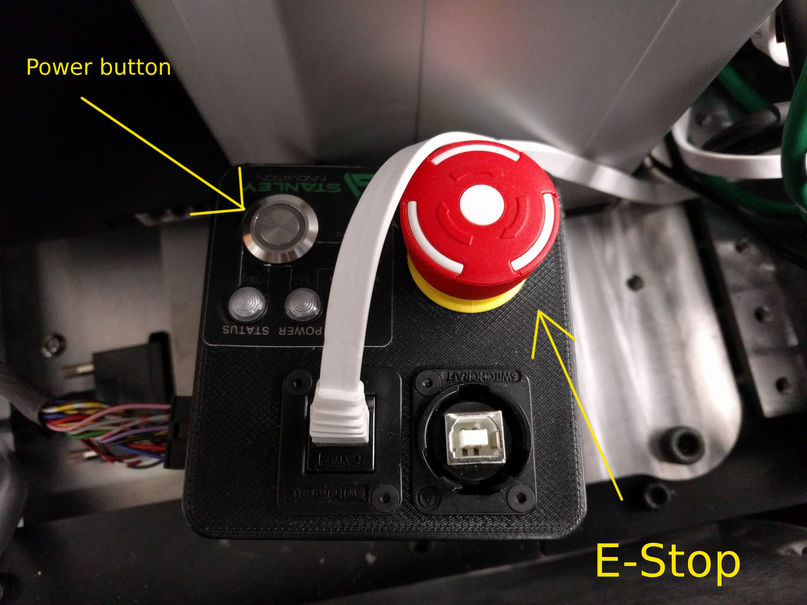
\includegraphics[width=300px]{figures/base_power.jpg}
  \caption{The Segway base control box}
  \label{fig:base_powerbox}
\end{figure}

During boot up and boot down, the base emits a tone that lets you know systems are normal. You can also verify the lights on the control box. 

\begin{figure}[h] 
  \centering
  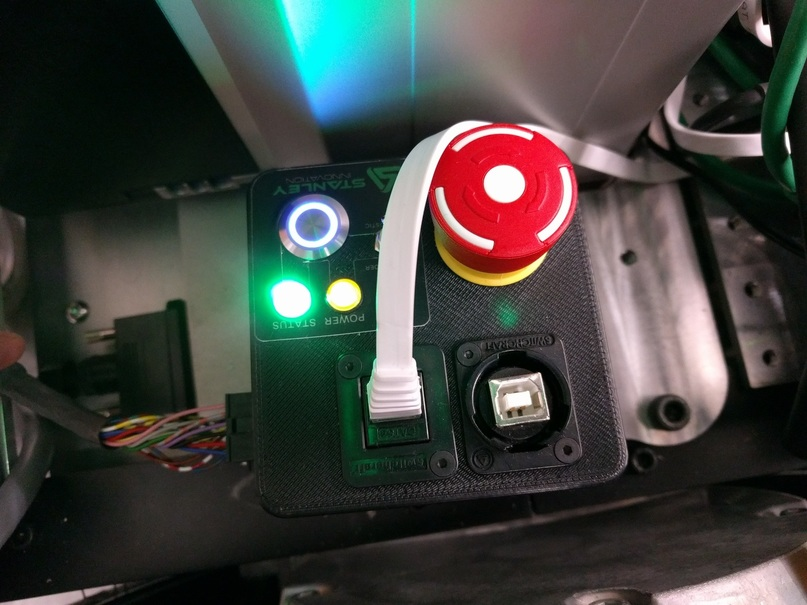
\includegraphics[width=300px]{figures/base_power_on.jpg}
  \caption{The control box power button is pulsing slowly and the indication LED is green. Both indicate system has booted normally.}
  \label{fig:base_powerbox_on}
\end{figure}

\subsubsection{PCs- Poli1 and Poli2}
The PCs also turn on at the press of a button. Since they use power supplied by the base, the base must already be turned on before attempting to power the PCs.\\

See Figure \ref{fig:computer_1_power} and Figure \ref{fig:computer_2_power} for help finding the power buttons. The power button on each computer should light up once powered.

\begin{figure}[h] 
  \centering
  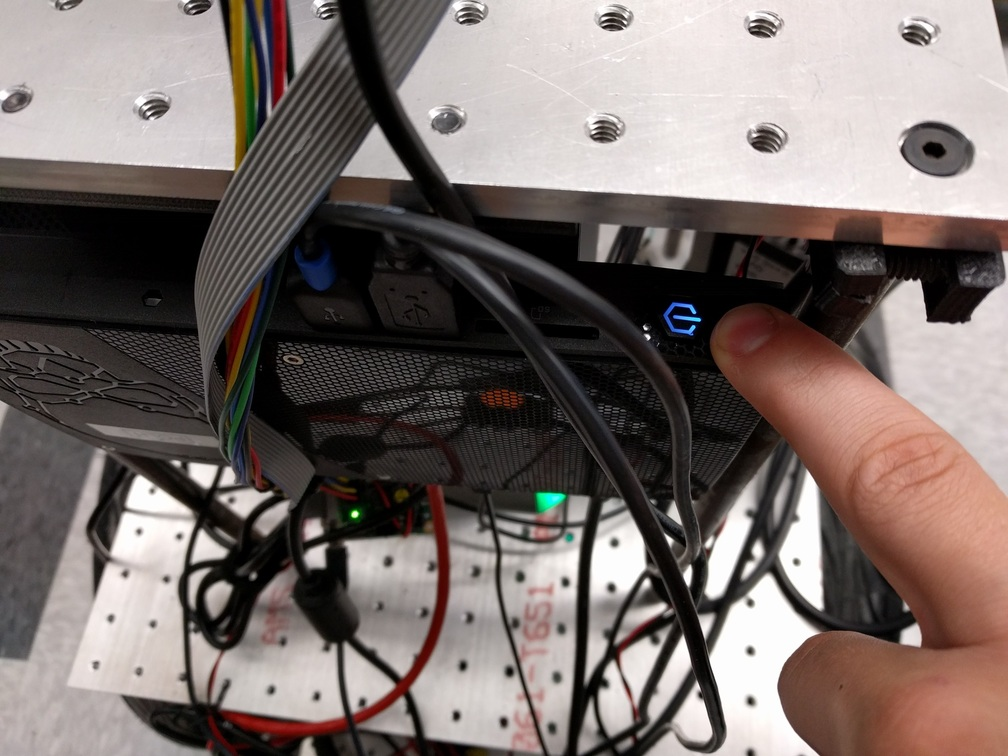
\includegraphics[width=300px]{figures/computer_1_power.jpg}
  \caption{Location of the power button for PC1.}
  \label{fig:computer_1_power}
\end{figure}

\begin{figure}[h] 
  \centering
  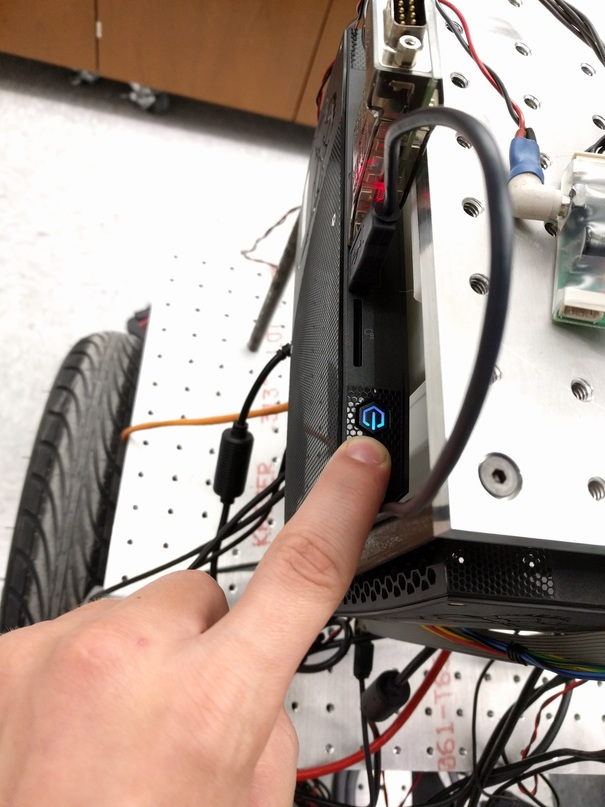
\includegraphics[height=300px]{figures/computer_2_power.jpg}
  \caption{Location of the power button for PC2.}
  \label{fig:computer_2_power}
\end{figure}

\clearpage

\subsubsection{Arm}
Since the arm is back-drivable when unpowered, it is sometimes advantageous to turn the arm off manually and move it to a safe position. If the previous operator has done this, you will want to check if the arm's power button is active. \\

Locate the arm's access panel- with power and USB inputs. The power button also exists on this panel. The arm is powered if you cannot move it or if its holding its own weight without falling.

\begin{figure}[h!] 
  \centering
  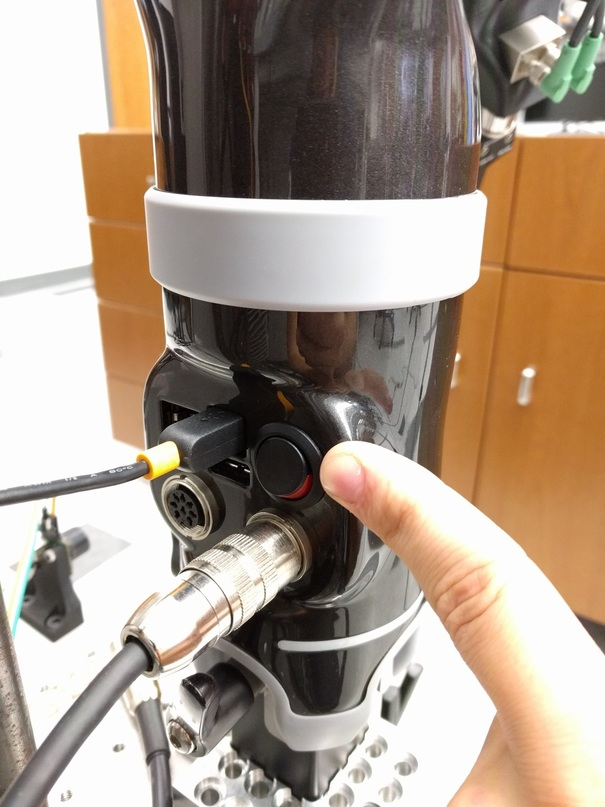
\includegraphics[height=300px]{figures/arm_power.jpg}
  \caption{Location of the power button for the Kinova Jaco2. In this case, the arm is on.}
  \label{fig:arm_power}
\end{figure}

\subsection{Turning off the robot}
This basically happens in the reverse sequence of turning the robot on. \\

First you should confirm the safety of the arm position and turn it off manually if necessary. See Figure \ref{fig:arm_power} for the power button location. \\

Secondly, the PCs should be soft-shutdown, if possible. This means running the \texttt{sudo shutdown now} command in a terminal in a ssh session with the PC. If necessary, you can hold down the power button to shut the PC down. \\

Lastly, press the base's powerbutton on its control box. An audible tone should sound, and the LED should blink red. It will be fully powered down in around a minute.

\subsection{Charging the robot}\label{sec:charging_robot}
The robot charges through a high voltage, VGA style connection directly into the base (see Figure \ref{fig:base_charger}). The cable is held into the base through two thumb-screws.

\begin{figure}[h!] 
  \centering
  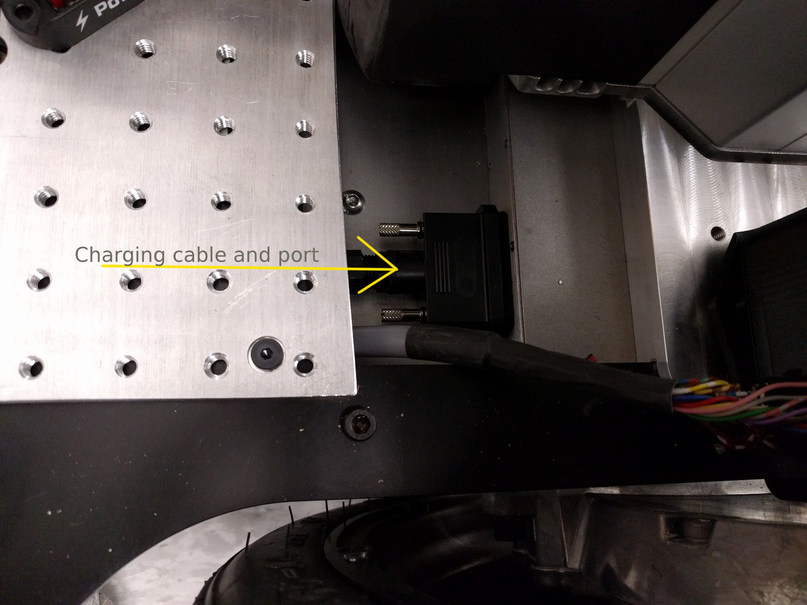
\includegraphics[width=250px]{figures/base_charging_cable_top.jpg}
  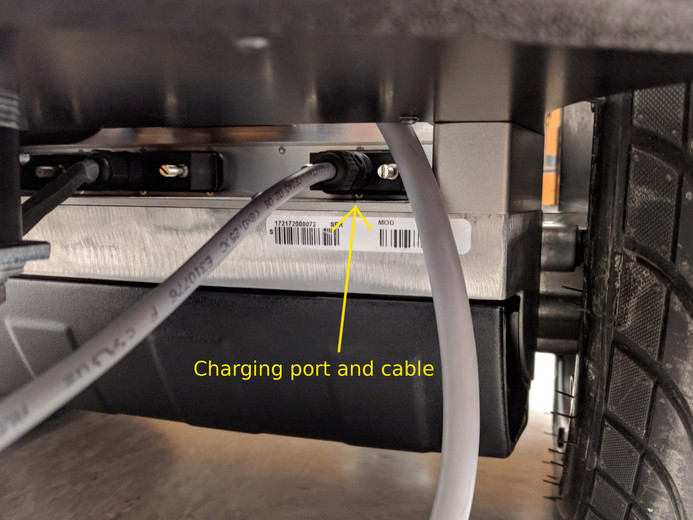
\includegraphics[width=250px]{figures/base_charging_cable_bottom.jpg}
  \caption{Top and bottom view of the charging cable connector for the Segway RMP.}
  \label{fig:base_charger}
\end{figure}

\clearpage

\textbf{\textcolor{red}{NOTE}} It is important that the charger be turned \textbf{OFF} when un/plugging the charging cable to the base. It is also important than the cable be inserted evenly, and not at an angle. Either of these can cause a momentary short and can tax the charger.

\begin{figure}[h!] 
  \centering
  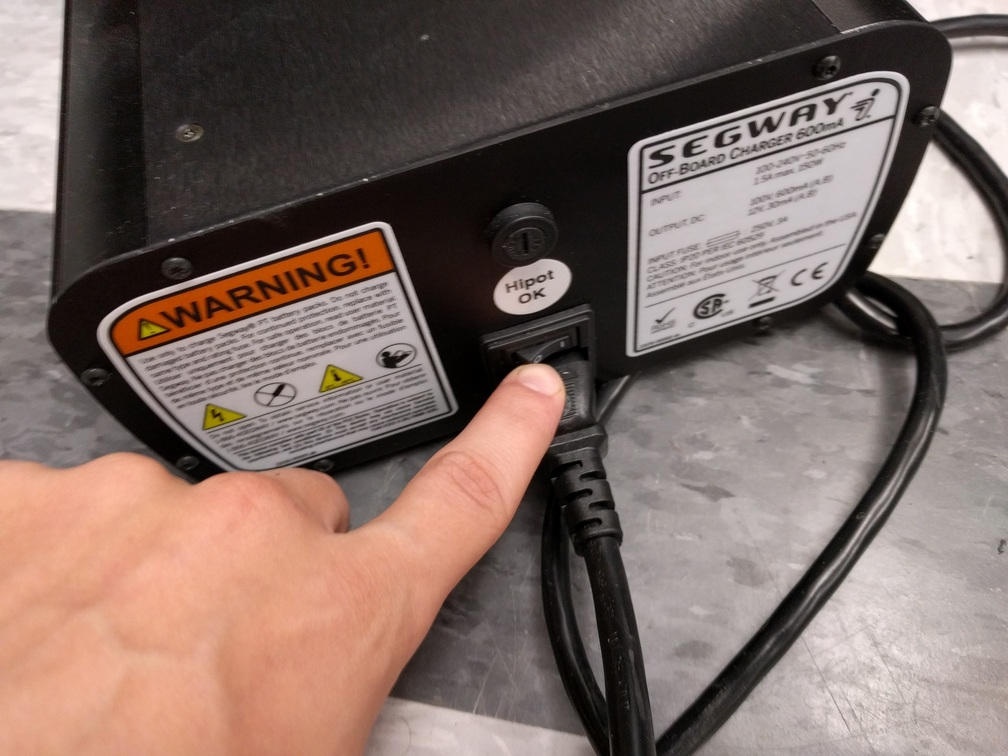
\includegraphics[width=250px]{figures/base_charger_turn_on.jpg}
  \caption{Back view of the Segway base charger. The charger's power switch is indicated.}
  \label{fig:base_charger_power}
\end{figure}

\subsection{Disconnecting robot from charger}
Turn the charger off using its power switch on its back panel. Unthread the thumb screws from the connector and the base. Pull the charging cable backwards, off the connector, with even force.

See Figure \ref{fig:base_charger} and Figure \ref{fig:base_charger_power} for details. 


\section{Create user accounts}\label{sec:user_accounts}
\subsection{Setting up local hosts file}
Examples in this section make use of a hostname alias, rather than specifying the IP address of \textbf{poli1}. 
To add \textbf{poli1} and \textbf{poli2} as hostnames, see Example \ref{ex:host_file}. 
This should already be done on the robot's computers but will need to be done for any computer used to access the robot's computers or network. 

\begin{example}{Example of setting hosts file for robot use}
  \label{ex:host_file}
  On your local computer (assuming Ubuntu)
  \begin{itemize}
    \item Open \texttt{/etc/hosts} with sudo privileges 
	\item Add \texttt{10.66.171.91 poli1}
    \item Add \texttt{10.66.171.24 poli2}
    \item Save and exit
  \end{itemize}
  IP addresses are assumed to be set according to Section \ref{sec:network_configuration}
\end{example}

\subsection{Initial Account Setup}
Connect to the robot's wireless network, which should be of the form \texttt{PoliV2-N}, where N is a number designating the enumeration of that particular robot. It is brought up when the router boots, which takes a couple minutes after turning on the robot. Since the robot needs to be powered for this, go ahead and look through Section \ref{sec:turn_on_hardware} to turn the robot on. \\

You can connect to the network using the password \textbf{simachines}. 
This same password is used for access to the default accounts on \textbf{poli1} and \textbf{poli2} computers.

We will now go through the process of adding a user account with the correct permissions to one of the PCs, \textbf{poli1}.

\begin{example}{Example of setting up user account on poli1}
  \label{ex:user_accounts}
  \begin{itemize}
  	\item ssh into poli1: \texttt{ssh poli@poli1}
    \item Make yourself a user: \texttt{sudo adduser <your desired username>}
    \item Add user to groups: \texttt{sudo usermod -aG sudo,dialout,cdrom,adm,dip,plugdev,lpadmin,sambashare,audio <your username>}
	\item  Log off: \texttt{exit}
    \item Set up your ssh keys for your new user: \texttt{ssh-copy-id <your user>@poli1}
	\item Log in to your new user account: \texttt{ssh <your user>@poli1}
  \end{itemize}
\end{example}

Now, log into your account and create a catkin workspace in your home directory. You can see how to do that at \\
\href{http://wiki.ros.org/catkin/Tutorials/create_a_workspace}{http://wiki.ros.org/catkin/Tutorials/create\_a\_workspace}.

If successful, do the same processes for \textbf{poli2}. Don't forget to setup your bash environment as in Example \ref{ex:bashrc_poli1}, \ref{ex:bashrc_poli2}.\\

\begin{example}{Setting up initial .bashrc file: POLI1}
  \label{ex:bashrc_poli1}
    Open \texttt{\textasciitilde/.bashrc} \\
    At the bottom add \texttt{source \textasciitilde/catkin\_ws/devel/setup.bash} \\
    Save and close \\
    In a terminal enter the command: \texttt{source \textasciitilde/.bashrc}
\end{example}

\begin{example}{Setting up initial .bashrc file: POLI2}
  \label{ex:bashrc_poli2}
    Open \texttt{\textasciitilde/.bashrc} \\
    At the bottom add \texttt{source \textasciitilde/catkin\_ws/devel/setup.bash} \\
    At the bottom add \texttt{source poli\_RMP.bash} \\
    At the bottom add \texttt{export ROS\_MASTER\_URI=http://poli1:11311} \\
    Save and close \\
    In a terminal enter the command: \texttt{source \textasciitilde/.bashrc}
\end{example}

Finally, you need to setup wireless internet under your user on \textbf{poli1} and \textbf{poli2}. 
This requires logging in by connecting a keyboard, mouse and monitor directly to the robot and setting up a connection to a network through Ubuntu's \texttt{network manager}. \\

There exist specific WiFi accounts for the robots to connect to the \texttt{utexas} network. Contact a lab manager for these credentials.

If \texttt{network manager}'s front face is updated to be X-forwarded or you switch to a different manager, you may be able to set up the wifi connection in a terminal via \texttt{ssh}.


\section{Setting up the code base}
\textbf{Note: This section of the guide is possibly outdated. Please see \href{https://github.com/si-machines/poli2/wiki}{the software wiki} for the latest.} \\

There are a fair number of forks and specific branches that need to be checked out to get all systems working.
Luckily the ROS-install system makes fetching these simple.

\subsection{Fetch high level repository}

\begin{example}{Setting up the PoliV2 codebase}
  \label{ex:poli2_codebase_setup}
  Assuming catkin\_ws is initialized and using a PoliV2 computer. \\
  \begin{itemize}
    \item \texttt{git clone https://github.com/si-machines/poli2.git} in \texttt{src} of catkin\_ws
    \item cd into root of \texttt{catkin workspace}
    \item \texttt{rosdep update}
    \item \texttt{rosdep install -{}-from-paths src -{}-ignore-src -{}-rosdistro=kinetic -y}
    \item \texttt{cd \textasciitilde/catkin\_ws/src} 
	\item \texttt{wstool init ./ ./poli2/dependencies.rosinstall}
    \item \texttt{sudo apt-get purge ros-kinetic-dynamixel-workbench-toolbox}
    \item \texttt{cd \textasciitilde}/catkin\_ws
    \item \texttt{catkin\_make}
  \end{itemize}
  In the future you can update from all repos using the \texttt{wstool update} command.
\end{example}


We use \texttt{rosdep} to fetch packages on the public repository list (reading from \texttt{package.xml}) and \texttt{wstool} to fetch specific branches of specific forks as specified in the \texttt{.rosinstall} file.

Note that the codebase should be set up on both \textbf{poli1} and \textbf{poli2}, so repeat Example \ref{ex:poli2_codebase_setup} on both PCs. \\

\textcolor{red}{Important note:} The last thing needed is to copy the \texttt{poli\_RMP.bash} file to the root of your home directory. 
This file is required by the \texttt{segway\_ros} driver. \\
As long as Examples \ref{ex:setup_rmp_env} and \ref{ex:bashrc_poli2} have been followed, the RMP environment variables should be set in perpetuity. 

\begin{example}{Setup RMP Environment Variables}\label{ex:setup_rmp_env}
\begin{itemize}
  \item \texttt{roscd poli\_launch}
  \item \texttt{cp config \textasciitilde/poli\_RMP.bash }
  \item \texttt{source \textasciitilde/.bashrc}
\end{itemize}
\end{example}



\section{Starting ROS and critical systems}
Since PoliV2 is a multi-purpose research platform, and will be used by many separate users, there are no assumptions made about the virtual environment.
As such, no \textit{\textbf{device}} launch files are brought up on startup or log-in; though the ability to do this is fully supported. See 'Automating Bringup Procedure` Section on the \href{https://github.com/si-machines/poli2/wiki/How-To}{Poli2 Wiki}.\\


However, a single launch file is brought up on startup to start the \textbf{ros core}. This is to prevent accidental preemption of the core, and to allow some (typically) persistent parameters to remain on the roscore session, e.g. robot\_description. \\



Thus, with the robot's systems on and the codebase installed and compiled, we're ready to bring up the systems manually.

\subsection{Poli1 PC}
As detailed in Section \ref{sec:network_configuration}, each PC can only bring up the devices it has connected to it, plus any networked components. 

We can bring up all poli1's devices as in Example \ref{ex:poli1_bringup}.

\begin{example}{Bringup poli1's devices}
  \label{ex:poli1_bringup}
    \texttt{ssh user@poli1} \\
  \texttt{roslaunch poli\_launch poli1\_bringup.launch}
\end{example}

\subsection{Poli2 PC}
We can bring up all poli2's devices as in Example \ref{ex:poli2_bringup}.
\texttt{poli2\_bringup.launch} does the heavy lifting, bringing up the navigation stack, MoveIt!, and all networked components. \\

\begin{example}{Bringup poli2's devices}
  \label{ex:poli2_bringup}
  \texttt{ssh user@poli2} \\
  \texttt{roslaunch poli\_launch poli2\_bringup.launch} \\
  Wait several seconds \\
  \texttt{roslaunch poli\_launch scan\_merger.launch}
\end{example}

Note that you must launch the scan\_merger.launch file after bringing up everything else on \textbf{poli2}. 
This is due to a bug in the implementation of the scan merger node. 
However, it is still necessary to run, due to the navigation stack's reliance on the merged tf frame that the scan merger provides. Otherwise, issues with the tf tree ensue. \\

Now all the robot's systems should be up. If you run into problems, check the troubleshooting page on the \href{https://github.com/si-machines/poli2/wiki}{poli2 high level repository} or in Chapter \ref{ch:troubleshooting} of this document. You can see specific examples of how to move components or access robot state in Chapter \ref{ch:componentspecifics}.

\subsection{Networking the Robot With Your Computer}
This allows you to run graphical elements (RViz, image\_view, etc) on your local machine that may be difficult or impossible to view on the robot's computers directly. \\

\begin{example}{Reserving IP on the robot's network} \label{ex:reserve_ip}
\begin{itemize}
  \item On your PC, connect to the desired robot's WiFi
  \item Go to the router's webpage: \texttt{10.66.171.1}
  \item Login
  \item Click \textbf{Advanced}
  \item Under \textbf{Network} in the navigation pane, select \textbf{DHCP server}
  \item There will be a table of MAC addresses and IP addresses...
  \item Find the \textbf{name} entry of your host and click \textbf{bind}.
  \item Copy the IP address that your machine is bound to.
\end{itemize}
\end{example}

\begin{example}{Setting up ROS Environment}\label{ex:setting_up_bashrc}
\begin{itemize}
  \item Edit your \texttt{\textasciitilde/.bashrc} file
  \item At the bottom add \texttt{export ROS\_IP=xyz} where \texttt{xyz} is the IP your machine is bound to on the network.
  \item At the bottom add \texttt{export ROS\_MASTER\_URI=http://poli1:11311}
  \item Save and close
  \item Source your .bashrc: \texttt{source \textasciitilde/.bashrc}
\end{itemize}
  In the event you want to run a roscore locally, simply change this file again, but where \texttt{ROS\_IP=127.0.0.1} and \texttt{ROS\_MASTER\_URI=http://localhost:11311}.
\end{example}

Example \ref{ex:reserve_ip} walks through binding your IP, which prevents getting kicked off the ROS network when your IP lease expires. 
Example \ref{ex:setting_up_bashrc} walks through setting up the environment variables needed to network through the robot. \\

Note that this would have to be done on each robot you want to work with, since each has its own network. 
Therefore it will be easier to reserve the same IP address on each robot network, preventing you from needing to update your \texttt{\textasciitilde/.bashrc} with each new robot. \\


You can read more about ROS networking at \href{http://wiki.ros.org/ROS/NetworkSetup}{http://wiki.ros.org/ROS/NetworkSetup}.

\chapter{Robot Organization}\label{ch:robot_organization}

\section{Network Configuration}\label{sec:network_configuration}
Each robot has its own local area network (LAN) that facilitates connectivity of components and computation. 

Not all components are hardwired to the network; some must be connected to a PC via USB.
As such, the components connected directly to a PC are local to that PC and can only be brought up on that PC. See Figure \ref{fig:network_map} for details on the connectivity of the system.


\begin{figure}[]
\centering
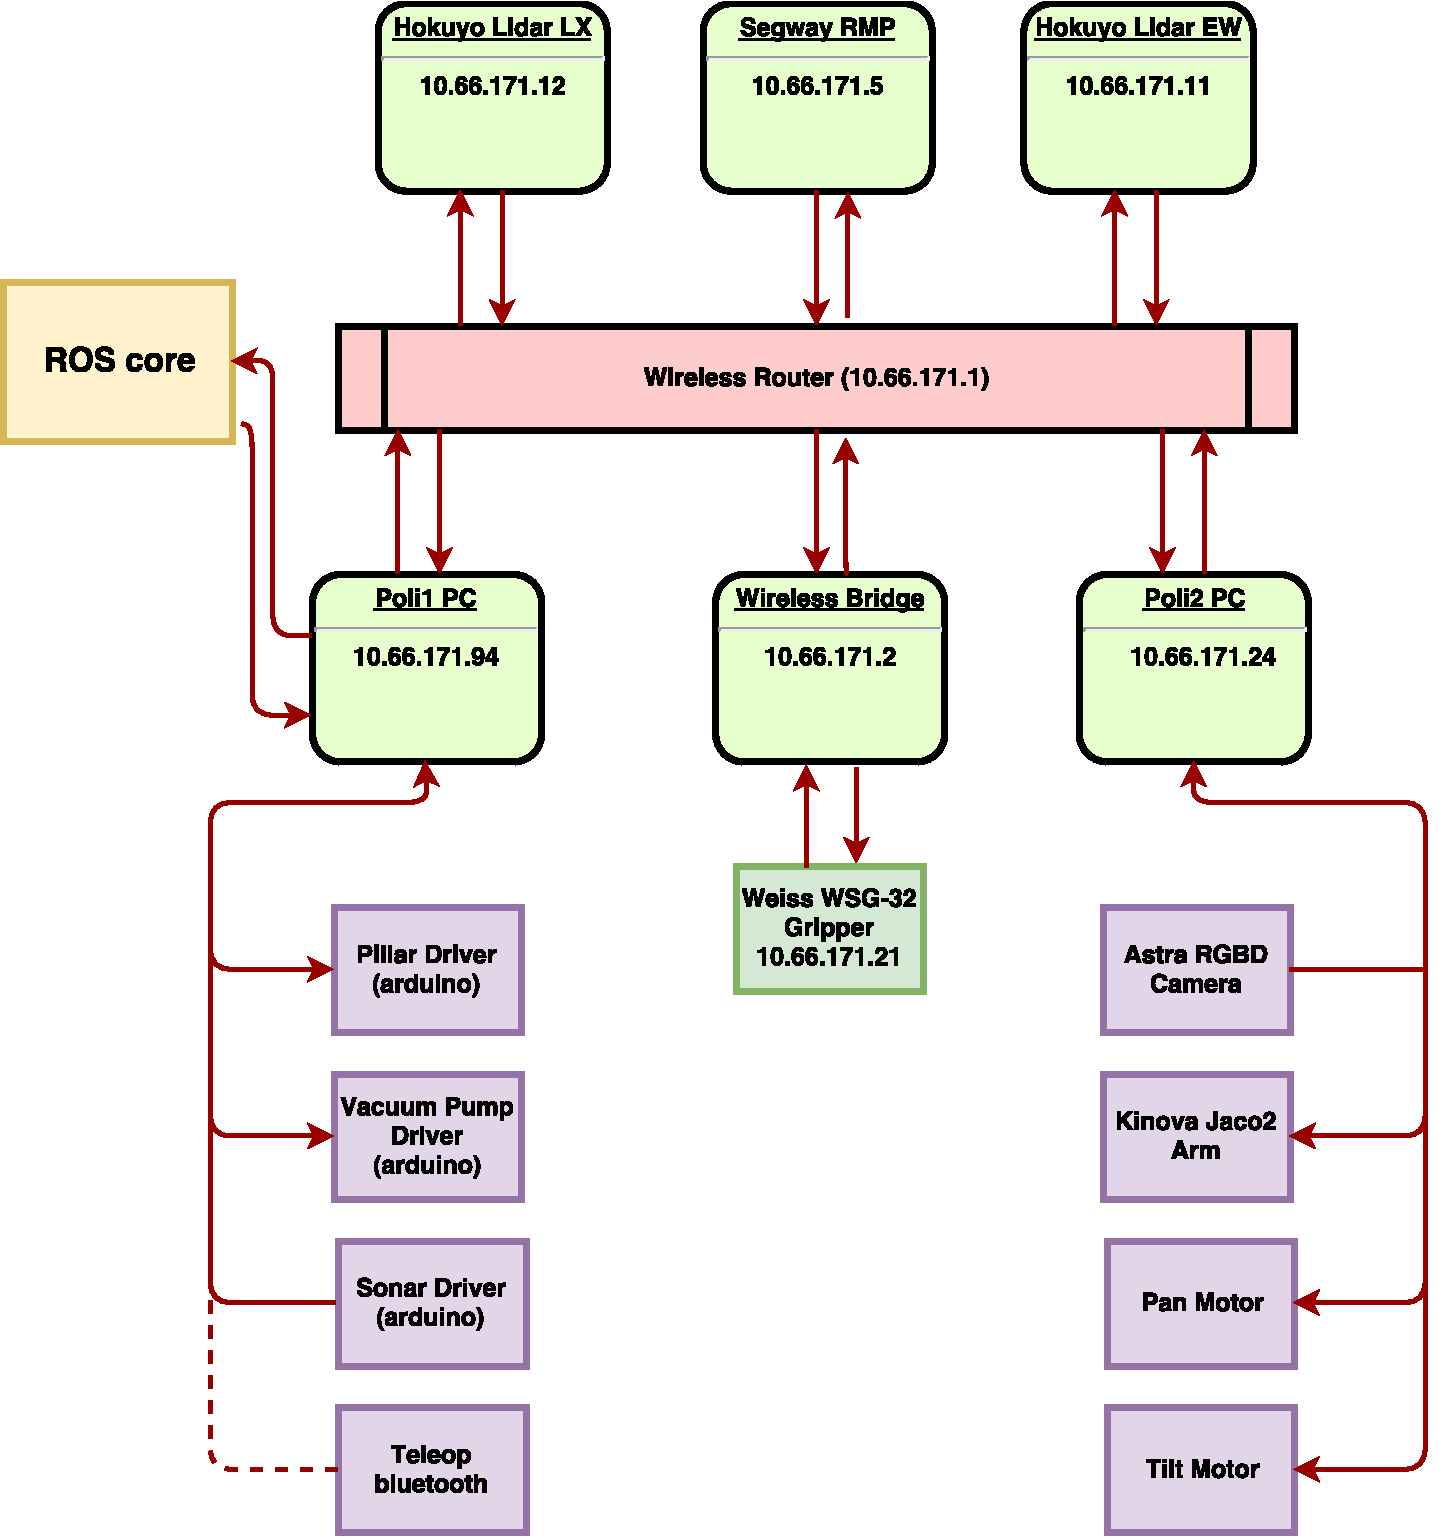
\includegraphics[width=425px]{figures/network_diagram_cropped.pdf}
\caption{Network map for the PoliV2 Robot Platform}
\label{fig:network_map}
\end{figure}

\section{Codebase}
At the time of this writing, the codebase depends heavily on forks and branches of existing opensource packages and libraries. 
This section briefly looks at which fork/branch combination is used and why it was made. \\

Note that fork/branch resolution happens automatically through \texttt{wstool} and that this section is for informational purposes only.

\begin{itemize}
   \item segway\_v3 - Stanley Innovation - \texttt{master} : no kinetic release
   \item wsg\_32\_description - SI-Machines - \texttt{master} : no kinetic release
   \item ira\_laser\_tools - iralabdisco - \texttt{master} : no kinetic release
   \item kinova\_ros - GT-RAIL - \texttt{7dof\_kinetic} : no kinetic release + 7dof changes. Follows \texttt{7dof} branch of same fork.
   \item wsg50-ros-pkg - SI-Machines - \texttt{kinetic-devel} : no kinetic release; URDF and driver bug fixes.
   \item epos\_hardware - RIVeR-Labs - \texttt{kinetic-devel} : no kinetic release
   \item dynamixel-workbench - ROBOTIS-GIT - \texttt{master} : Kinetic release is broken
   \item dynamixel-workbench-msgs - ROBOTIS-GIT - \texttt{master} : Kinetic release is broken
\end{itemize}

\subsection{Microcontroller development}
All microcontroller components are arduino IDE compatible. 
All files used to flash onto the particular arduino can be found in \href{https://github.com/si-machines/poli2/tree/master/poli2_launch/scripts/arduino}{\texttt{scripts/arduino/}} folder of the \texttt{poli\_launch} package. \\

A guide on how to do development and flash to Arduinos is available at the github wiki: \href{https://github.com/si-machines/poli2/wiki/Arduino-Development}{https://github.com/si-machines/poli2/wiki/Arduino-Development}. \\

Note that the Arduino devices names are given in Figure \ref{fig:network_map}. These device names are definite for the first Poli2 robot, but may change on subsequent robots depending on how device names are assigned.

\subsection{Microcontroller wiring diagrams}
\subsubsection{LED + limit switch}
\begin{figure}[h]
\centering
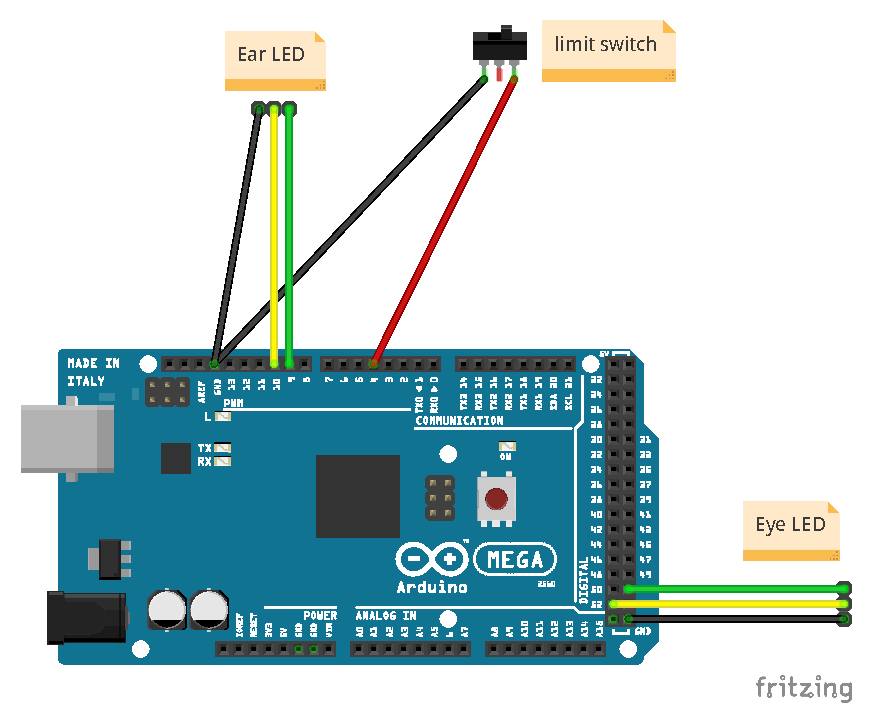
\includegraphics[width=250px]{figures/head_arduino_bb.pdf}
\caption{Wiring diagram for the LED and limit switch arduino}
\label{fig:head_arduino}
\end{figure}

\subsubsection{Pillar}

\subsubsection{Vacuum}


\chapter{Setting up a New Robot}\label{ch:setting_up_new_robot}
This section contains all information pertaining to setting up and configuring the components of the robot as they come from the factory. 
These changes are strictly software configuration necessary for the components to communicate and would only need to be carried out once per robot.

\section{Setting up Network Components}
The Segway RMP base is set in the 10.66.171.x sub net. This requires us to change all other networked devices (router, lasers, computers) to accept being addressed in this range. For simplicity, we try to keep all IP addresses consistent across all robots. Reference Figure \ref{fig:network_map} when setting the IPs of the various components.

\subsection{Setting up network hosts}
In order to resolve network names and communicate over a common network, both \textbf{poli1} and \textbf{poli2} need each others names resolved. See example \ref{ex:network_hosts}

\begin{example}{Configure network hosts}\label{ex:network_hosts}
  \begin{itemize}
    \item On \textbf{poli1}
    \item Edit \texttt{/etc/hosts} with \texttt{sudo}
    \item Add \texttt{10.66.171.24 poli2}
    \item Save and exit
    \item On \textbf{poli2}
    \item Edit \texttt{/etc/hosts} with \texttt{sudo}
    \item Add \texttt{10.66.171.91 poli1}
    \item Save and exit
  \end{itemize}
\end{example}

\subsection{Setting up the connections in Ubuntu}
Example \ref{ex:network_manager} is required to simultaneously use Internet via WiFi and LAN via ethernet. 
This manually manages the ethernet connection that allows connection to the LAN and prevents Ubuntu from using it as an outbound route.

\begin{example}{Configuring Ubuntu's network manager}\label{ex:network_manager}
	 \texttt{ auto lo \\
 iface lo inet loopback \\
 auto eno1 \\
 iface eno1 inet static \\
 address 10.66.171.x\\
 netmask 255.255.255.0}
   \begin{itemize}
     \item Edit \texttt{etc/network/interfaces} file with \texttt{sudo}
     \item Fill in the file with the above codeblock
     \item Change the IP address after \texttt{address} to match the IP of the computer whose file you're editing. 
     \item Restart computer.
   \end{itemize}
\end{example}

\subsection{Setting up network connections for the router}
When setting up the main router, change the router's IP address to \texttt{10.66.171.1}. \\

While you're there, change the network name to something appropriate (SSID = PoliV2-N) where N == a number that won't cause collisions with existing robot networks. \\

Finally, go to the DHCP client table. Here you will be able to bind IP addresses of important components. You will need to bind the IPs of the wireless bridge, \texttt{poli1} and \texttt{poli2} at a minimum. \\

\subsection{Change the IP Addresses of the lasers}
The default IP address of the Hokukyo lasers are 192.168.0.10 \\

You can find a link to the Windows IP changing tool provided by Hokuyo in Section \ref{sec:sensor_data_sheets}. 
The ROS \texttt{urg\_node}, which is what we use to fetch data from the lasers, also has a node called \texttt{change\_ip\_address}. 
This has not been tested by our group, but may work in place of the Windows tool. \\

Change the laser IPs to the appropriate value. 
Ensure the correct laser gets the expected IP address.

\subsection{Configure the Gripper's IP}
Next, configure the Gripper's IP to be statically 10.66.171.21. 
This can be accomplished through the gripper's web interface at its default IP address, \texttt{192.168.1.20}. 

This should be done outside the immediate network, though, if you've already changed the IP range of the router.



\subsection{Configure the Gripper's Wireless Bridge}
Finally, configure the wireless bridge to be a client of the router and reset its IP range.
The bridge has a default IP address of \texttt{192.168.1.1}.

\begin{example}{Reconfiguring the wireless bridge}
  \begin{itemize}
    \item Connect to bridge's LAN interface
    \item Navigate to \texttt{Quick Setup} on the left navigation panel
    \item Click Next
    \item Select \textbf{Client} under `At Home'
    \item Click Next
    \item Select the local router SSID for the robot you're configuring
    \item Enter the correct security credentials
    \item Finish. Results in a reboot.
    \item Select \textbf{Network} on the left navigation panel
    \item Select \textbf{Static IP} for type
    \item Enter \textbf{10.66.171.2} for IP address
    \item Enter \textbf{10.66.171.1} for the gateway
  \end{itemize}
\end{example}


\chapter{Component Specifics}\label{ch:componentspecifics}
This chapter details the particulars of each component. This includes how to interface with the component through the high level repository \href{https://github.com/si-machines/poli2}{Poli2} and its dependent packages and libraries. 

\section{Sensors}
\subsection{Lidar}
The lidar are used for both localization and obstacle detection. 
In order to use multiple scan sources for localization using existing algorithms, they are merged into a single scan using \texttt{ira\_laser\_tools}. 
This package has a bug in implementation that requires the merging node be launched after the lidar drivers are brought up. \\

\subsection{Sonar}
The sonar are used strictly for obstacle detection and have a range of approximately 5 feet at their current mounting points. 
As it stands, the sonar are better used for clear and reflective surfaces that the lidar cannot pickup. 
Cliff detection is not possible with the current configuration of sonars.

\section{Manipulation}
Arm-based manipulation has two hardware components due to the use of a third party gripper (WSG-32) with the manipulator (Jaco2 7DOF). These components are exposed to ROS separately. We also consider the pan-tilt motor system which, though have different controllers, are exposed to ROS under the same interface ros-control. 

\subsection{Jaco2 7DOF}
The Jaco2 uses the same ROS driver that previous Kinova products use. So most things (services, actions, messages) should be familiar. 
Do note that we use the \texttt{kinetic\_7dof} branch of the GT-RAIL fork of \texttt{kinova\_ros}, and that any finger services in the API will not work with the third party gripper.

\subsubsection{Arm Driver}
The majority of the driver functions are identical for the 7dof Jaco. 
The most obvious change is the name of the arm as shown as a prefix for all driver topics and services. \\

The arm has been configured for gravity compensation to be used in an upright position with the third party gripper. 
Changing either of these parameters would necessitate changing the driver's gravity vector and regenerating center of mass parameters.

\begin{example}{Start gravity compensation}
  \label{ex:start_gravity_compensation}
    \texttt{rosservice call /j2s7s300\_driver/in/start\_force\_control "\{\}"} \\
    Note that the 'start\_grav\_comp` service doesn't seem to do anything.
\end{example}

\subsubsection{Arm MoveIt! Configurations}
There exist two separate MoveIt! configurations for the custom Jaco2 arm: \\
\texttt{jaco2\_custom\_arm\_moveit\_config} and \texttt{poli2\_full\_config}. \\

The former is a standalone configuration for the arm and the Weiss gripper, useful when running manipulation on a table top. 
The latter is a configuration which takes into account the entire PoliV2 robot platform and is thus collision-aware of the robot's components. \\

The \texttt{poli2\_full\_config} is run by default in the startup launch files. \\
\texttt{jaco2\_custom\_arm\_moveit\_config} is kept only as a useful addition.


\subsection{Vacuum Gripping Unit}
There is a ROS-controllable vacuum unit that would allow high level vacuum manipulation plans. 
This unit is controlled by an arduino-based microcontroller and is connected to \textbf{poli1} via USB. \\

Since this unit may or may not always be installed to the robot, ensure that the box is plugged into a \textbf{12V} power rail. \\
See Example \ref{ex:vacuum_gripper} for how to command the gripper system.

There are three commands that the interface accepts. 
\begin{itemize}
\item Start pump: begins pulling a vacuum
\item Stop pump: stops pulling a vacuum
\item Release object: Requires the pump be running. Briefly stops pulling vacuum long enough to release an object that gripper may be holding.
\end{itemize}

\begin{example}{Start vacuum unit}
  \label{ex:vacuum_gripper}
    \texttt{rosservice call /poli/gripper\_vacuum "command: 0"} \\
    Find the mappings of commands in the \href{https://github.com/si-machines/poli2/blob/master/poli_msgs/srv/GripperPump.srv}{GripperPump.srv} service description file in \texttt{poli\_msgs}.
\end{example}



\subsection{Weiss WSG-32 Gripper}
The Weiss gripper has a number of services and a single control topic.
Here are several examples of commanding the gripper through ROS. \\

The gripper is wirelessly interfaced through the network and is accessible through a web interface. 
Navigating to the address \texttt{10.66.171.21}, the Gripper's IP address, should bring up the gripper's landing page. 
This page allows manual control of position, debugging and settings management.

Occasionally the gripper may run into a fault that must be manually cleared. 
You can clear the fault through the web interface or as in Example \ref{ex:gripper_fault_ack}.

\begin{example}{Send position goal to Gripper}
  \label{ex:gripper_pos_goal}
    \texttt{rostopic pub /wsg\_50\_driver/wsg/goal\_position std\_msgs/Float64 "data: 0.0"} \\
    
    The mode can be left blank, but velocity must be non-zero. \\
    Units are in mm. \\
    Max range is ~65 mm. Min range is 0mm.
\end{example}

\begin{example}{Clearing a gripper fault}
  \label{ex:gripper_fault_ack}
  TODO
\end{example}

\subsection{Pan-tilt}
The pan and tilt motors are controlled through \texttt{ros\_controllers} position controllers. 
Thus they are both controlled through ROS in the same way.

\begin{example}{Send position goal to pan motor}
  \label{ex:pan_pos_goal}
    \texttt{rostopic pub /pan\_motor/position\_controller/command std\_msgs/Float64 "data: 0.0"} \\
\end{example}

\begin{example}{Send position goal to tilt motor}
  \label{ex:tilt_pos_goal}
    \texttt{rostopic pub /tilt\_motor/position\_controller/command std\_msgs/Float64 "data: 0.0"} \\
\end{example}

\textcolor{red}{\textbf{IMPORTANT NOTE}}: The tilt motor utilizes relative encoders to detect the position of the motor. 
This means the reference position, i.e. zero position of the tilt motor is exactly the motor position when the motor initially gets power. 
If the tilt motor is not started in the correct position, the model will not reflect reality, since the URDF model assumes a particular location for the zero position. 
\textcolor{red}{This becomes especially important for perception purposes, where the angle must be known}.

\section{Platform}
The base platform has one lower level method of control: velocity. 
You can publish velocity commands directly to the base through \texttt{rostopic} (see Example \ref{ex:base_velocity}). \\

Generally, the base will be controlled through one of two means: teleop and/or autonomous navigation. 
Navigation is handled via \texttt{movebase} and can be activated via 2D navigation goals. 
See more on this at \href{http://wiki.ros.org/move_base}{http://wiki.ros.org/move\_base}.

\begin{example}{Publish velocity to base}
  \label{ex:base_velocity}
    \texttt{rostopic pub /poli/teleop/cmd\_vel geometry\_msgs/Twist MSG}\\
\end{example}

\begin{example}{Starting base teleop with playstation controller}
  \label{ex:base_teleop}
    Pre: Bringup procedures on both PCs have been completed according to Ex \ref{ex:poli1_bringup} and Ex \ref{ex:poli2_bringup}. \\
    \texttt{ssh poli1} \\ 
    \texttt{roslaunch poli\_navigation\_apps playstation\_teleop.launch} \\

\end{example}


\section{Computers}
Each computer has a defacto account named \texttt{poli}, which can be used in a pinch. 
However, proper procedure is to create and use your own user account on each computer, as detailed in Section \ref{sec:user_accounts}. \\

It should be assumed that poli1 will automatically bring up the \texttt{roscore} under the \texttt{poli} user account, which has sudo privileges. 
This prevents the ROS network from being killed accidentally, but means that ROS parameters can persist beyond a node's session which is problematic in certain situations. \\



\chapter{Data Sheets}\label{ch:datasheets}
Many components are off the shelf and have their own specific documentation.

Here we provide links to the item's technical data sheets and third party repositories if applicable.
\section{Data Sheets}
\subsection{Sensors} \label{sec:sensor_data_sheets}
\subsubsection{Hokuyo 30EW}
\href{http://www.robotshop.com/media/files/pdf2/utm-30lx-ew_specification.pdf}{Specifications} \\
\href{http://www.robotshop.com/media/files/pdf2/utm-30lx-ew_product_overview.pdf}{Overview}
\href{http://www.robotshop.com/media/files/pdf/communication-protocol-utm-30lx-ew.pdf}{Communication Protocol} \\
\href{http://wiki.ros.org/urg_node}{Code repository} \\
\href{http://www.robotshop.com/content/ZIP/ip-changer-utm-30lx-ew.zip}{Windows IP changer}
\subsubsection{Hokuyo 10LX}
\href{http://www.robotshop.com/media/files/zip/documentation-ust-10lx.zip}{All documentation} \\
\subsubsection{Maxbotix 1230EZ}
\href{https://www.maxbotix.com/documents/XL-MaxSonar-EZ_Datasheet.pdf}{Specfications} \\
\href{https://www.maxbotix.com/tutorials1/016-maxsonar-quick%E2%80%91start-guide.htm}{Quick-start Guide} \\

\subsubsection{Orbecc Astra}
\href{https://orbbec3d.com/product-astra/}{Specifications} \\
\href{http://wiki.ros.org/astra_camera}{Code repository} 

\subsection{Manipulation}
\subsubsection{Jaco2 7DOF}
\href{http://www.kinovarobotics.com/wp-content/uploads/2017/04/JACO-7-Spherical-DOF-Technical-Specifications.pdf}{Specifications} \\
\href{http://www.kinovarobotics.com/wp-content/uploads/2017/06/JACO%C2%B2-User-Guide-Asstive-Robotics-April-2017.pdf}{User guide} \\
\href{http://www.kinovarobotics.com/wp-content/uploads/2017/04/JACO-7-Spherical-DOF-Advanced-Guide.pdf}{Advanced guide} \\
\href{https://github.com/GT-RAIL/kinova-ros/tree/7dof_kinetic}{Code repository} \\

\subsubsection{Weiss WSG-32 Gripper}
\href{https://www.weiss-robotics.com/wp-content/uploads/wsg32_manual.pdf}{Manual} \\
\href{https://www.weiss-robotics.com/wp-content/uploads/wsg_command_set_reference_manual-4-0-0.pdf}{Command set} \\
\href{https://github.com/si-machines/wsg50-ros-pkg/tree/kinetic_devel}{Code repository} \\
\href{http://wiki.ros.org/wsg_32_description}{Description repository} \\

\subsection{Base Platform}
\subsubsection{RMP 110}
\href{https://github.com/StanleyInnovation/segway_v3}{Code repository}

\chapter{Troubleshooting}\label{ch:troubleshooting}

\section{Acceptable errors}

\subsection{Base}
\subsubsection{Hector Pose Estimation}
\texttt{Skipping XML Document /opt/ros/kinetic/share/\\
hector\_pose\_estimation/hector\_pose\_estimation\_nodelets.xml which had no Root Element.  This likely means the XML is malformed or missing.} \\

This will show when launching the base. We don't use hector pose estimation, so this does not affect anything.

\subsection{Arduino}
\subsubsection{Lost connection}
\texttt{Lost sync with device, restarting...} \\

This shows up periodically, for a yet-to-be-determined reason. It does not seem to negatively affect input/output from the arduino(s).

\section{Connectivity and Hardware Issues}
\subsection{Dynamixel driver crashes}
This is almost always a conflict with USB devices. Theoretically the \texttt{udev} rules should eliminate the issue (these exist in \texttt{poli\_launch/config}). \\
Unfortunately the only answer currently is to un/plug the USB2Dynamixel adapter and restart the driver.

\subsection{Gripper not connected}
Exact error: `Unable to connect, please check the port and address used' \\

Whats wrong: The gripper is not connected to the network. Try power cycling the arm. Unfortunately something internal to the gripper is preventing it from connecting. This happens with DHCP and a static IP on the gripper.

\subsection{Gripper connected but does not respond to position goals}
Exact error: TODO \\

Whats wrong: The gripper has likely hit a fault as a protection mechanism. 
To continue with normal operation, the fault needs to be acknowledged. 
An example of how this can be done is in Example \ref{ex:gripper_fault_ack}.

Note: Due to a limitation in the design of the gripper-arm circuit pair, the gripper frequently hits a Fast Stop error. A solution for this is in the works.


\subsection{TF tree broken / no laser scans output in RViz / localization fails}
Exact error: `No laser scan received (and thus no pose updates have been published) ' \\

Whats wrong: The scan merger node was launched before the lidar drivers were fully up, or it wasn't launched at all. Running \texttt{rosrun poli\_launch scan\_merger.launch} in a separate terminal solves this.


\section{Issues with existing code bases}

More specific issues that arise coming from other packages or libraries should be opened as issues on the respective issue tracker. \\

Issues or additions to the PoliV2 repository should be opened as a ticket at \href{https://github.com/si-machines/poli2/issues}{https://github.com/si-machines/poli2/issues} or as a Pull Request.
  
\end{document}